\documentclass[aspectratio=169,t,dvipdfmx,12pt]{beamer}
\mode<presentation>
\setbeamersize{text margin left=8mm,text margin right=8mm}
\setbeamertemplate{headline}{}
\setbeamertemplate{navigation symbols}{}
\setbeamertemplate{footline}{%
 \hbox{\noautospacing\noautoxspacing
       \hbox to \paperwidth{\hss
       \vbox to 10pt{%
       \hbox{\insertframenumber{} / \inserttotalframenumber}\vss}%
       \hspace*{4pt}}}}

\setbeamertemplate{title page}{%
 \vbox{}%
 \vfill\begin{centering}
  \begin{beamercolorbox}[sep=8pt,left]{title}
   \usebeamerfont{title}\inserttitle\par
   \ifx\insertsubtitle\relax\else
    \vskip0.25em
    {\usebeamerfont{subtitle}\usebeamercolor[fg]{subtitle}\insertsubtitle\par}%
   \fi
  \end{beamercolorbox}%
  \begin{beamercolorbox}[sep=8pt,left]{author}
   \usebeamerfont{author}\insertauthor
  \end{beamercolorbox}
  \begin{beamercolorbox}[sep=8pt,left]{institute}
   \usebeamerfont{institute}\insertinstitute
  \end{beamercolorbox}
  \begin{beamercolorbox}[sep=8pt,left]{date}
   \usebeamerfont{date}\insertdate
  \end{beamercolorbox}\vskip0.5em
  {\usebeamercolor[fg]{titlegraphic}\inserttitlegraphic\par}%
 \end{centering}
 \vskip 0pt plus 1filll
 {\quad\tiny Copyright Katsuhiro Ueno.}
}

\mode<all>

\usepackage[deluxe,nomacro]{otf}% for HiraKakuPro-W6
\usepackage{txfonts}% for math fonts
\renewcommand{\sfdefault}{phv}
\renewcommand{\rmdefault}{ptm}
%\renewcommand{\ttdefault}{cmtt}
\renewcommand{\familydefault}{\sfdefault}
\renewcommand{\kanjifamilydefault}{\gtdefault}
\setbeamerfont{title}{size=\large,series=\bfseries}
\setbeamerfont{subtitle}{size=\small,series=\bfseries}
\setbeamerfont{frametitle}{size=\large,series=\bfseries}
\setbeamerfont{author}{size=\small}
\setbeamerfont{institute}{size=\small}
\setbeamerfont{date}{size=\small}
\usefonttheme{professionalfonts}% use my own font settings
\setlength\unitlength{1mm}
\setbeamertemplate{enumerate items}[default]
\setbeamercolor{block title}{fg=white, bg=blue!70!black}
\setbeamercolor{block body}{fg=black, bg=blue!10!white}
%------

\usepackage{tikz}
\usetikzlibrary{calc}
\usetikzlibrary{overlay-beamer-styles}

\usepackage[absolute,overlay]{textpos}
\setlength{\TPHorizModule}{1mm}
\setlength{\TPVertModule}{1mm}
\textblockorigin{0mm}{0mm}
\setlength{\unitlength}{1mm}

\newcommand\codestyle{%
  \ttfamily
  \chardef\{=`\{
  \chardef\}=`\}
  \chardef\_=`\_
  \chardef\~=`\~
  \chardef\/=`\\
  \frenchspacing}
\newcommand\code[1]{\texttt{\protect\codestyle #1}}
\newenvironment{prog}
  {\codestyle\begin{tabbing}}
  {\end{tabbing}}

\definecolor{KW}{rgb}{0.7, 0.0, 0.7}
\newcommand\KW[1]{{\color{KW}#1}}
\newcommand\ST[1]{{\color{KW}#1}}
\definecolor{ID}{rgb}{0.0, 0.2, 0.8}
\newcommand\ID[1]{{\color{ID}#1}}

\definecolor{focus}{rgb}{1.0, 0.0, 0.3}
\newcommand\focus[1]{{\color{focus}\underline{#1}}}

\definecolor{comment}{rgb}{0.1, 0.5, 0.2}
\newcommand\comment[1]{{\color{comment}(* {\normalfont #1} *)}}
\newcommand\Func{\rightarrow}
\newcommand\Pair{\times}%\mathrel{\code{*}}}

\newcommand\TITLE[1]{\bigskip\hspace{-14pt}\structure{\large\bfseries #1}}

\newcommand\smlsharp{SML\#}
\newcommand\denote[1]{[\![ #1]\!]}

\newcommand\PART[1]{%
  \begin{frame}
  \vfill\hfil\structure{\Large\bfseries #1}
  \end{frame}}

\newcommand\vbar{~\mid~}

\newcommand\infer[2]{\begin{tabular}{c}#1\relax\\\hline#2\end{tabular}}
\newcommand\inferB[2]{\begin{tabular}[b]{c}#1\relax\\\hline#2\end{tabular}}
\newcommand\inferNamed[4]{%
{\def\temp{#1}\ifx\temp\empty\else\parbox{50pt}{\hfill(\temp)}\hspace{6pt}\fi}%
\infer{#2}{#3}%
{\def\temp{#4}\ifx\temp\empty\else\hspace{6pt}\temp\fi}%
}

%------
\title{\smlsharp{}コンパイラを速くする:\\
タスク並列、末尾呼び出し、部分評価機構の開発}
\author{上野雄大}
\date{2025年6月15日 関数型まつり}

\begin{document}

\maketitle

\begin{frame}{自己紹介}

上野雄大(うえのかつひろ)
\begin{itemize}
\item 2004年 学生として\smlsharp{}コンパイラの開発に参加
\item 2009年 職業として\smlsharp{}コンパイラの開発に従事
\item 2025年現在:\begin{tabular}[t]{@{}l}新潟大学自然科学系准教授\\(専門:計算機科学,ソフトウェア工学)\end{tabular}
\end{itemize}

\bigskip

関数型言語開発歴21年(うち職業として16年)
\begin{itemize}
\item \smlsharp{}開発歴≒\smlsharp{}使用歴
\item \smlsharp{} is 人生
\item 大堀淳先生(\smlsharp{}プロジェクト代表者)には感謝しかない
\end{itemize}

\bigskip

{\footnotesize
SNS(というかオンラインコミュニケーション全般)が苦手ですすみません…}

\end{frame}

\begin{frame}{\smlsharp{}とは}
Standard MLを包摂する日本発のフルスケール関数型言語.

\bigskip

MLを「MLに閉じない世界」で実現する
\begin{itemize}
\item C言語とのシームレスな相互運用
\item 既存のハードウェア・ソフトウェア資源をそのまま活用
\item マシンネイティブなデータ表現
\item OSネイティブなマルチスレッドサポート
\item C言語と同様の分割コンパイルとリンク
\item 強力なレコード演算(多相レコード,自然結合)
\item SQLとの統合
\item 動的型によるJSONの型付き操作
\end{itemize}
\bigskip
詳しくは\url{https://smlsharp.github.io/}をチェック
\end{frame}

\begin{frame}{今日のおはなし:関数型言語を「作る」視点}

\begin{itemize}
\item マルチコアCPUでベストパフォーマンスを出す(3.6.0〜)
\item Aarch64対応(4.2.0〜)
\item 部分評価に基づくコードの最適化(4.2.0〜)
\end{itemize}

\bigskip

これらの開発経験を題材に,関数型言語処理系を作る視点を共有したい.
\begin{itemize}
\item どんな問題に対して,何を狙い,何をしたのか
\end{itemize}

\pause\bigskip

すべて\smlsharp{} 4.2.0(2025年3月リリース)で試せます.
\begin{itemize}
\item ぜひ使ってみてね!
\end{itemize}

\end{frame}

\begin{frame}{\smlsharp{}コンパイラアーキテクチャ}

{\small
\begin{tikzpicture}[y=0.8cm,anchor=north west]
\draw[alt=<1>{white}{dashed,fill=yellow,thick}] (2.5,0.2) -- ++(11.6,0) -- ++(0,-7.6) -- ++(-14.3,0) -- ++(0,6) -- ++(14.3-11.6,0) -- cycle;
\draw[alt=<1>{white}{dashed,fill=green!30,thick}] (5.3,-7.8) rectangle (7.6,-9);
\draw[alt=<1>{white}{dashed,fill=red!10,thick}] (11,-7.8) rectangle (14.1,-9);
\node[draw] (SML) at (0,0) {\smlsharp{}言語};
\only<2->{
\node[draw,fill=white,label=south:{\scriptsize Absyn}] (Absyn) at (3,0) {抽象構文木};
\node[draw,fill=white,label=south:{\scriptsize PatternCalc}] (Pattern) at (7,0) {コア言語};
\node[draw,fill=white,label=300:{\scriptsize IDCalc}] (ID) at (10,0) {変数スコープなし言語};
\node[draw,fill=white,label=south:{\scriptsize TypedCalc}] (Typed) at (11,-2) {型付き言語};
\node[draw,fill=white,label=south:{\scriptsize TypedLambda}] (Lambda) at (5.5,-2) {型付きラムダ計算の一種};
\node[draw,fill=white,label=300:{\scriptsize RecordCalc}] (Record) at (0,-2) {型抽象を関数化した言語};
\node[draw,fill=white,label=south:{\scriptsize BitmapCalc}] (Bitmap) at (0,-4) {データ表現が明確な言語};
\node[draw,fill=white,label=south:{\scriptsize ClosureCalc}] (Closure) at (5,-4) {高階関数のない言語};
\node[draw,fill=white,label=300:{\scriptsize RuntimeCalc}] (Runtime) at (9.5,-4) {多相性が限定された言語};
\node[draw,fill=white,label=south:{\scriptsize ANormal}] (Anormal) at (9,-6) {評価順序を明示する言語};
\node[draw,fill=white,label=300:{\scriptsize MachineCode}] (Machine) at (.5,-6) {メモリ操作を明示する言語};
\node[draw,fill=white,label=south:{\scriptsize LLVMIR}] (LLVM) at (0,-8) {SSA形式(LLVM中間表現)};
}
\node[draw,fill=white] (Target) at (8,-8) {機械語};
\only<1>{
\draw[-latex,dashed] (SML) -- node[above right]{???} (Target);
}
\only<2->{
\draw[-latex] (SML) -- (Absyn);
\draw[-latex] (Absyn) -- (Pattern);
\draw[-latex] (Pattern) -- (ID);
\draw[-latex] (ID) -- (Typed);
\draw[-latex] (Typed) -- (Lambda);
\draw[-latex] (Lambda) -- (Record);
\draw[-latex] (Record) -- (Bitmap);
\draw[-latex] (Bitmap) -- (Closure);
\draw[-latex] (Closure) -- (Runtime);
\draw[-latex] (Runtime) -- (Anormal);
\draw[-latex] (Anormal) -- (Machine);
\draw[-latex] (Machine) -- (LLVM);
\draw[-latex] (LLVM) -- (Target);
\node[anchor=center] at (6,-1.6) {\textbf{\smlsharp{}コンパイラ}};
\node at (5.8,-7.7) {\textbf{LLVM}};
\node at (11,-7.8) {\textbf{\smlsharp{}ランタイム}};
\draw[latex-latex,ultra thick] (Target) -- node[below]{リンク} ++(2.3,0);
}
\end{tikzpicture}}

\end{frame}

\PART{マルチコアCPUでベストパフォーマンスを出す}

\begin{frame}{\smlsharp{}はC言語との連携が得意}

様々なC関数を\smlsharp{}にそのままインポートできる.

インポートしたC関数にはMLの関数型が付く.

データ変換なしに\smlsharp{}の値(文字列や配列など)をC関数に渡せる.

\bigskip

\begin{prog}
\# \pause \KW{val} \ID{puts} = \_import \ST{"puts"} : string -> int;\\\pause
val puts = fn : string -> int\\
\# \pause puts \ST{"Hello"};\\\pause
Hello\\
val it = 10 : int\\
\# \pause app (ignore \KW{o} puts) [\ST{"Hello"}, \ST{"World"}];\\\pause
Hello\\
World\\
val it = () : unit\\
\#
\end{prog}

\end{frame}

\begin{frame}{\code{pthread\_create}も直接呼べる}

\begin{prog}
\KW{fun} \ID{spawn} f =\\
~~~~\KW{let}\\
~~~~~~\KW{val} 'a\#boxed \ID{pthread\_create} =\\
~~~~~~~~~~\focus{\_import "pthread\_create"}\\
~~~~~~~~~~: (unit ptr ref, unit ptr, 'a -> unit ptr, 'a) -> int\\
~~~~~~\KW{val} \ID{r} = ref (Pointer.NULL ())\\
~~~~~~\KW{fun} \ID{callback} f = (f (); Pointer.NULL ())\\
~~~~\KW{in}\\
~~~~~~pthread\_create (r, Pointer.NULL (), callback, f);\\
~~~~~~!r\\
~~~~\KW{end}
\end{prog}

{\footnotesize
(同様の関数が\code{Pthread.Thread.create}として標準提供されている)}

\end{frame}

\begin{frame}{細粒度スレッドライブラリMassiveThreadsを使ってタスク並列}

MassiveThreadsならスレッドを山ほど作れる.

\begin{prog}
\KW{fun} \ID{fib} 0 = 0\\
~~| \ID{fib} 1 = 1\\
~~| \ID{fib} n = \alt<1>{\phantom}{}{\KW{if} n < 16 \KW{then}} \alt<1>{}{\underline}{fib (n - 1)} + \alt<1>{}{\underline}{fib (n - 2)} \alt<1>{\phantom}{}{\KW{else}}\\
~~~~~~~~~~~~\alt<1>{\phantom}{}{\KW{let} \KW{val} \ID{t} = Myth.Thread.create (\KW{fn} () => \underline{fib (n - 2)})}\\
~~~~~~~~~~~~\alt<1>{\phantom}{}{\KW{in} \underline{fib (n - 1)} + Myth.Thread.join t}\\
~~~~~~~~~~~~\alt<1>{\phantom}{}{\KW{end}}
\end{prog}

\bigskip

\only<3->{
純粋な再帰関数とタスク並列は相性がいい
\begin{itemize}
\item \underline{\code{fib (n - 1)}}の計算と\underline{\code{fib (n - 2)}}の計算は互いに独立だよね
\item それぞれの計算を別の物理コアで独立に並列実行したら倍速で終わるよね
\item …本当に?
\end{itemize}
}
\end{frame}

\begin{frame}{ボトルネック:ガベージコレクション(GC)}

計算を進めるにはヒープからのメモリの供給が必要.

\begin{prog}
\KW{fun} \ID{fib} 0 = 0\\
~~| \ID{fib} 1 = 1\\
~~| \ID{fib} n = \KW{if} n < 16 \KW{then} fib (n - 1) + fib (n - 2) \KW{else}\\
~~~~~~~~~~~~\KW{let} \KW{val} \ID{t} = Myth.Thread.create (\focus{fn () => fib (n - 2)})\\
~~~~~~~~~~~~\KW{in} fib (n - 1) + Myth.Thread.join t\\
~~~~~~~~~~~~\KW{end}
\end{prog}

この関数クロージャは
\begin{itemize}
\item グローバルなヒープのどこかにアロケートされ,
\item \code{Myth.Thread.create}によってどこかのCPUと共有され,
\item 不要になったら自動的に回収されなければならない
\end{itemize}

\bigskip

大域的なGCがスレッド間に暗黙の相互依存を生み出してしまう….

\end{frame}

\begin{frame}{世界を止めない並行並列GC}

\smlsharp{}からマルチコアCPUの並列計算性能を最大限に活用するためには,
大域的な資源管理をしながらもスレッドを止めないGCが必要.
\begin{itemize}
\item stop-the-worldなどもってのほか
\item GC都合のメモリ競合も最小限に
\end{itemize}

\bigskip

\smlsharp{}のGCは世界を止めない並行並列GC
\begin{itemize}
\item 全てのスレッドがミューテータにもコレクタにもなる
\item 全体の統括者や同期をせずにグローバルな状態管理をする
\item 世界を止めずにルートセット列挙
\item スレッド数1のときはほぼ普通のマークスイープGC
\end{itemize}

\end{frame}

\begin{frame}{世界を止めないGCの難しさ}

GCが成立するには「ある瞬間」における「ルートセット全体」と
「そこから到達可能なオブジェクト集合」の両方が必要.

\bigskip

世界を止めずにこれらを入手できるか?

\bigskip

\begin{enumerate}
\item トレーシングの最中にオブジェクトグラフが書き換わる
\begin{itemize}
\item[→]\normalsize Yuasaのスナップショットライトバリアで
オブジェクトグラフ全体のスナップショットを取る.
\end{itemize}
\bigskip
\item 全スレッドのルートセットを同時取得できない
\begin{itemize}
\item[→]\normalsize LevanoniとPetrankのスヌーピングライトバリアで
ルートセット列挙のタイムラグを埋める.
\end{itemize}
\end{enumerate}

\end{frame}

\begin{frame}{Yuasaのスナップショット}

ミューテータがポインタを書き換えるとき,古いポインタの値を覚える
(スナップショットライトバリア)ことで,
ライトバリアを有効にした時点のオブジェクトグラフを保存する.

\begin{center}
\begin{tikzpicture}
\only<21>{}
\draw (0,0) circle[x radius=0.6, y radius=2];
\draw (1,-2.2) rectangle (8,2.2);
\node[anchor=south west] at (-0.5,2.2) {\color{red}\strut
\alt<2-18>{mark}{\alt<19-20>{sweep}{}}};
\node[anchor=south west] at (1,2.2) {\strut
stack:
\only<3>{A}%
\only<4>{AB}%
\only<5-6>{AD}%
\only<7>{ADJ}%
\only<8>{ADI}%
\only<9-13>{ADH}%
\only<14>{ADHF}%
\only<15>{ADH}%
\only<16>{AD}%
\only<17>{A}%
};
\node[draw,thick,align=center,alt=<3-19>{alt=<18-19>{fill=orange}{fill=yellow}}{}] (A) at (2,1.5) {A};
\node[draw,thick,align=center,alt=<4-19>{alt=<5-19>{fill=orange}{fill=yellow}}{}] (B) at (1.8,0) {B};
\only<10->{\node[draw,thick,align=center,alt=<-19>{fill=orange}{}] (C) at (2.2,-1.5) {C};}
\node[draw,thick,align=center,alt=<5-19>{alt=<17-19>{fill=orange}{fill=yellow}}{}] (D) at (3.6,0.4) {D};
\only<-19>{\node[draw,thick,align=center] (E) at (3.4,-1) {E};}
\node[draw,thick,align=center,alt=<14-19>{alt=<15-19>{fill=orange}{fill=yellow}}{}] (F) at (5,1) {F\\};
\only<-19>{\node[draw,thick,align=center] (G) at (5,-1) {G};}
\node[draw,thick,align=center,alt=<9-19>{alt=<16-19>{fill=orange}{fill=yellow}}{}] (H) at (6.5,-1.5) {H};
\node[draw,thick,align=center,alt=<8-19>{alt=<9-19>{fill=orange}{fill=yellow}}{}] (I) at (5.8,0) {I};
\node[draw,thick,align=center,alt=<7-19>{alt=<8-19>{fill=orange}{fill=yellow}}{}] (J) at (7,1) {J};
\draw[-latex,thick] (0,0.75) --(A.north west);
\draw[-latex,thick] (0,0) --(B.north west);
\only<10->{\draw[-latex,thick] (0,-0.75) --(C.north west);}
\only<-13>{\draw[-latex,thick,alt=<13>{dotted}{}] (A) --(F.north west);}
\only<13->{\draw[-latex,thick] (A) --(B.north);}
\only<-11>{\draw[-latex,thick,alt=<11>{dotted}{}] (B) --(D.west);}
\only<11->{\draw[-latex,thick] (B) --(F.north west);}
\only<-19>{\draw[-latex,thick] (E) --(B.east);}
\draw[-latex,thick] (F) --(D.north east);
\only<-6>{\draw[-latex,thick,alt=<6>{dotted}{}] (F) --(J.north west);}
\only<6->{\draw[-latex,thick] (F) --(I.north);}
\draw[-latex,thick] (J) --(I.north east);
\draw[-latex,thick] (I) --(H.north);
\only<-19>{\draw[-latex,thick] (G) --(I.north west);}
\end{tikzpicture}
\end{center}

\end{frame}

\begin{frame}{Levanoni \& Petrankのスライディングビュー}

世界を止めないので,全スレッド同時にスナップショットライトバリアを
有効にしたり,ルートセット列挙したりできない.

\begin{center}
\begin{tikzpicture}
\node[draw] at (10,2.8){\alt<1>{理想}{現実}};
\draw[ultra thick,-latex] (0,0) --(11,0);
\draw[ultra thick,-latex] (0,2) --(11,2);
\node[anchor=south west] at (0,0) {Thread 2};
\node[anchor=south west] at (0,2) {Thread 1};
\only<1>{
\draw[dashed,thick] (3,-0.5) node[below] {$t$} --(3,2.5);
\draw[fill] (3,2) circle[radius=0.1];
\draw (3,2) --(3.4,2.4) --(6.5,2.4);
\node[anchor=south west] at (3.4,2.4) {snapshot, root};
\draw[fill] (3,0) circle[radius=0.1];
\draw (3,0) --(3.4,0.4) --(6.5,0.4);
\node[anchor=south west] at (3.4,0.4) {snapshot, root};
}
\only<2-3>{
\draw[dashed,thick] (3,-0.5) node[below] {$t_1$} --(3,2.5);
\draw[dashed,thick] (4,-0.5) node[below] {$t_2$} --(4,1);
\draw[dashed,thick] (7,-0.5) node[below] {$t_3$} --(7,2.5);
\draw[dashed,thick] (9,-0.5) node[below] {$t_4$} --(9,2.5);
\draw[fill] (3,2) circle[radius=0.1];
\draw (3,2) --(3.4,2.4) --(5.4,2.4);
\node[anchor=south west] at (3.4,2.4) {snapshot};
\draw[fill] (4,0) circle[radius=0.1];
\draw (4,0) --(4.4,0.4) --(6.4,0.4);
\node[anchor=south west] at (4.4,0.4) {snapshot};
\draw[fill] (7,2) circle[radius=0.1];
\draw (7,2) --(7.4,2.4) --(8.4,2.4);
\node[anchor=south west] at (7.4,2.4) {root};
\draw[fill] (9,0) circle[radius=0.1];
\draw (9,0) --(9.4,0.4) --(10.4,0.4);
\node[anchor=south west] at (9.4,0.4) {root};
\only<3>{
\draw[color=red,ultra thick,->] (7.2,1.5) --(8.8,1.5);
\draw[color=red,ultra thick] (9,2) circle[radius=0.3];
\node[anchor=north] at (8,1.5) {\color{red}snoop};
}
}
\end{tikzpicture}
\end{center}

代わりに,全スレッドのスナップショットライトバリアを確実に有効にしてから
ルートセットを列挙する.$t_3$と$t_4$のギャップは,
ポインタ書き換え時に新しいポインタの値を覚える
(スヌーピングライトバリア)ことで埋める.

\end{frame}

\begin{frame}{本当にこの戦略で動くのか…?}

並行並列プログラミングは人類の手に追えない…!
\begin{itemize}
\item 動かすたびに違うことが起こる
\item デバッガを使ったりデバッグプリントを入れると挙動が変わる
\item それでいて確実に動いてくれないと困る
\item 苦悶の跡:\url{https://github.com/smlsharp/smlsharp/blob/master/src/runtime/control.c}(2017行のうち1122行が日本語のコメント)
\end{itemize}

\bigskip

こんなときは…
\pause
\begin{center}\Large
数理モデルを立てて証明
\end{center}

\end{frame}

\begin{frame}{定理 [Ueno\&Ohori 2022]}
	Let thread $i$ $(1\le i\le n)$ enumerate its root set at $t_i$,
$t_0$ be any time before $t_i$, and
$t$ be $\mathop{\mathrm{max}}(t_1,\ldots,t_n)$.
	For any thread $i$ and time $t' \ge t$,
the following set $\mathcal{G}$ is disjoint with $\mathcal{R}(t')^*(\mathcal{S}_i(t'))$.
\[
\mathcal{G} = H \setminus T
\]
where
\begin{eqnarray*}
H &=& \mathcal{H}(t_0)\cup \mathcal{A}_1[t_0, t_1]\cup\cdots\cup \mathcal{A}_n[t_0,t_n],\only<2>{\hbox to 0pt{\vbox to 0pt{\vss\quad\fcolorbox{black}{yellow}{←回収範囲}\hss}}}\\
S &=& \mathcal{S}_1(t_1)\cup\cdots\cup \mathcal{S}_n(t_n),\only<2>{\hbox to 0pt{\vbox to 0pt{\vss\quad\fcolorbox{black}{yellow}{←ルートセット}\hss}}}\\
B &=& \mathop{\mathrm{snd}}(\mathcal{W}[t_0, t]) \cup \mathop{\mathrm{snd}}(\mathcal{D}[t_0, t]),\only<2>{\hbox to 0pt{\vbox to 0pt{\vss\quad\fcolorbox{black}{yellow}{←ライトバリア}\hss}}}\\
T &=& \mathcal{R}(t)^*(S \cup B).\only<2>{\hbox to 0pt{\vbox to 0pt{\vss\quad\fcolorbox{black}{yellow}{←トレース}\hss}}}
\end{eqnarray*}

\end{frame}

\begin{frame}{\smlsharp{}の並行並列GCアルゴリズム}

4つのシグナルをスレッド間で送りあってハンドシェーク
\begin{enumerate}
\item
	SYNC1: 2つのライトバリアをオン.これで$B$が手に入る.
	全スレッドがライトバリアをオンにした時点を$t_0$とする.
\item
	SYNC2: スレッドごとにルートセット列挙.これで$S$が手に入る.
	さらに現在のアロケーシ+ョンポインタを覚えることで$H$を手にいれる.
\item
	MARK: スレッドごとにスヌーピングライトバリアをオフにしてトレース.
$T$が手に入る.
\item
	ASYNC: $\mathcal{G}$を回収する.
\end{enumerate}

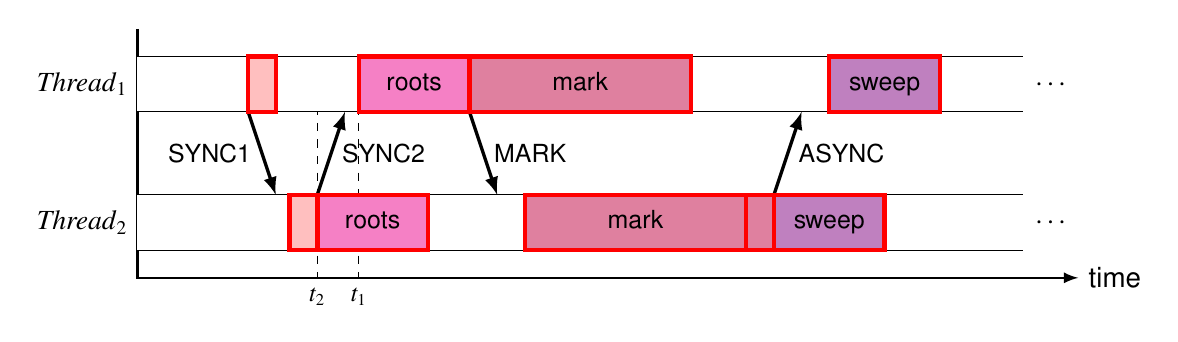
\begin{tikzpicture}[x=10pt,y=10pt]
\draw[thick,-latex] (0,9) --(0,0) --(34,0) node[right] {time};
\draw[dashed] (6.5,8) --(6.5,0) node[below] {\small $t_2$};
\draw[dashed] (8,8) --(8,0) node[below] {\small $t_1$};

\node[anchor=east] at (0,7) {$\mathit{Thread}_1$};
\fill[color=white] (0,6) rectangle(32,8);
\draw (0,6) --(32,6) (0,8) --(32,8);
\draw[very thick,-latex] (4,6) -- node[left]{\small SYNC1} (5,3);
\draw[ultra thick,color=red,fill=pink] (4,6) rectangle(5,8);
\draw[ultra thick,color=red,fill=magenta!50] (8,6) rectangle(12,8);
\node at (10,7) {\small\strut roots};
\draw[very thick,-latex] (12,6) -- node[right]{\small MARK} (13,3);
\draw[ultra thick,color=red,fill=purple!50] (12,6) rectangle(20,8);
\node at (16,7) {\small\strut mark};
\draw[ultra thick,color=red,fill=violet!50] (25,6) rectangle (29,8);
\node at (27,7) {\small\strut sweep};
\node at (33,7) {$\ldots$};

\node[anchor=east] at (0,2) {$\mathit{Thread}_2$};
\fill[color=white] (0,1) rectangle(32,3);
\draw (0,1) --(32,1) (0,3) --(32,3);
\draw[ultra thick,color=red,fill=pink] (5.5,1) rectangle(6.5,3);
\draw[very thick,-latex] (6.5,3) -- node[right]{\small SYNC2} (7.5,6);
\draw[ultra thick,color=red,fill=magenta!50] (6.5,1) rectangle(10.5,3);
\node at (8.5,2) {\small\strut roots};
\draw[ultra thick,color=red,fill=purple!50] (14,1) rectangle (22,3);
\node at (18,2) {\small\strut mark};
\draw[ultra thick,color=red,fill=purple!50] (22,1) rectangle (23,3);
\draw[very thick,-latex] (23,3) -- node[right]{\small ASYNC} (24,6);
\draw[ultra thick,color=red,fill=violet!50] (23,1) rectangle (27,3);
\node at (25,2) {\small\strut sweep};
\node at (33,2) {$\ldots$};
\end{tikzpicture}

\end{frame}

\begin{frame}{ベンチマーク(2022年(\smlsharp{} 3.6.0)時点}

\begin{center}
\begin{tabular}{cc}
mandelbrot & nqueen\\
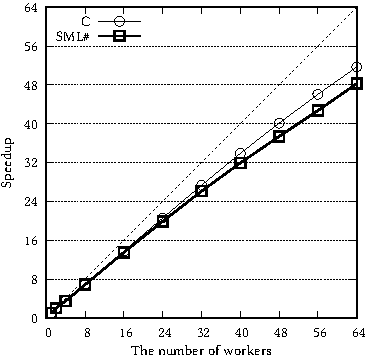
\includegraphics[height=6cm]{par_mandelbrot.pdf} &
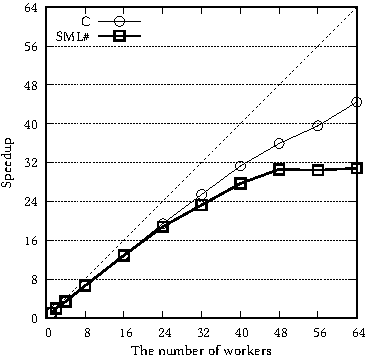
\includegraphics[height=6cm]{par_nqueen.pdf}
\end{tabular}

\medskip
{\scriptsize
評価環境:AMD EPYC 7501 2.0 GHz (32コア) $\times$ 2, 128 GB, Debian GNU/Linux 11}
\end{center}
\end{frame}

\PART{Aarch64対応}

\begin{frame}{ARM対応の何が問題?}

\begin{itemize}
\item[Q:] LLVMのターゲットを切り替えるだけでARMコード吐けるんじゃね?
\item[A:] 吐くだけならできます.動くかはなんとも…
\end{itemize}

\bigskip

動かない原因:
\begin{enumerate}
\item MassiveThreadsがARM対応してない → 2021年に解決
\item GCがARM対応してない? → 実はほぼ何もしなくてよかった(!)
\item 例外機構がARM対応してない? → amd64と同じItanium ABIだった
\item LLVMの末尾呼び出し最適化が効かない! → \textbf{今日の話題}
\item LLVMのnested functionが使えない! → (将来の課題)
\end{enumerate}

\bigskip

mod\_poppo氏によるApple Silicon対応\smlsharp{}の試み(Thanks!)
\begin{itemize}
\item \url{https://zenn.dev/mod_poppo/articles/smlsharp-aarch64-mac}
\end{itemize}

\end{frame}

\begin{frame}{末尾再帰とジャンプ}

\only<1>{
再帰呼び出しの後に計算が残っている=スタックを消費する(コール):
\begin{prog}
\KW{fun} \ID{sumList} nil = 0\\
~~| \ID{sumList} (h :: t) = \focus{sumList t} + h
\end{prog}
\begin{center}\small
\tikz\node[draw,align=left]{%
\code{\_\_SMLF7sumList:~~~~~~~~~~~~~~~~~~~~~~~~~}\\
\code{~~~~~~~~sub~~~~~sp, sp, \#48}\\
\code{~~~~~~~~cbz~~~~~x0, L4}\\
\code{~~~~~~~~ldr~~~~~w19, [x0]}\\
\code{~~~~~~~~ldr~~~~~x0, [x0, \#8]}\\
\code{~~~~~~~~\focus{bl~~~~~~\_\_SMLF7sumList}}\\
\code{~~~~~~~~add~~~~~w0, w0, w19}\\
\code{L4:~~~~~add~~~~~sp, sp, \#48}\\
\code{~~~~~~~~ret}};
\end{center}
}
\only<2>{
再帰呼び出しの後に計算が残っていない=スタックを消費しない(ジャンプ):
\begin{prog}
\KW{fun} \ID{loop} nil a = a\\
~~| \ID{loop} (h :: t) a = \focus{loop t (a + h)}\\
\KW{fun} \ID{sumList} l = \focus{loop l 0}
\end{prog}
\begin{center}\small
\tikz\node[draw,align=left]{%
\code{\_\_SMLF7sumList:~~~~~~~~~~~~~~~~~~~~~~~~~}\\
\code{~~~~~~~~sub~~~~~sp, sp, \#48}\\
\code{~~~~~~~~mov~~~~~w19, wzr}\\
\code{L2:~~~~~cbz~~~~~x0, L4}\\
\code{~~~~~~~~ldr~~~~~w9, [x0]}\\
\code{~~~~~~~~ldr~~~~~x0, [x0, \#8]}\\
\code{~~~~~~~~add~~~~~w19, w9, w19}\\
\code{~~~~~~~~\focus{b~~~~~~~L2}}\\
\code{L4:~~~~~mov~~~~~w0, w19}\\
\code{~~~~~~~~add~~~~~sp, sp, \#48}\\
\code{~~~~~~~~ret}};
\end{center}
}

\end{frame}

\begin{frame}{末尾呼び出し最適化が効かない}

\begin{itemize}
\item \smlsharp{}の末尾呼び出し最適化は自己末尾再帰を除いてLLVMに頼っていた
\item LLVMはARMターゲットにすると末尾呼び出しをジャンプにしてくれない
\item その結果,相互末尾再帰でスタックオーバーフロー
\end{itemize}

\begin{center}\footnotesize
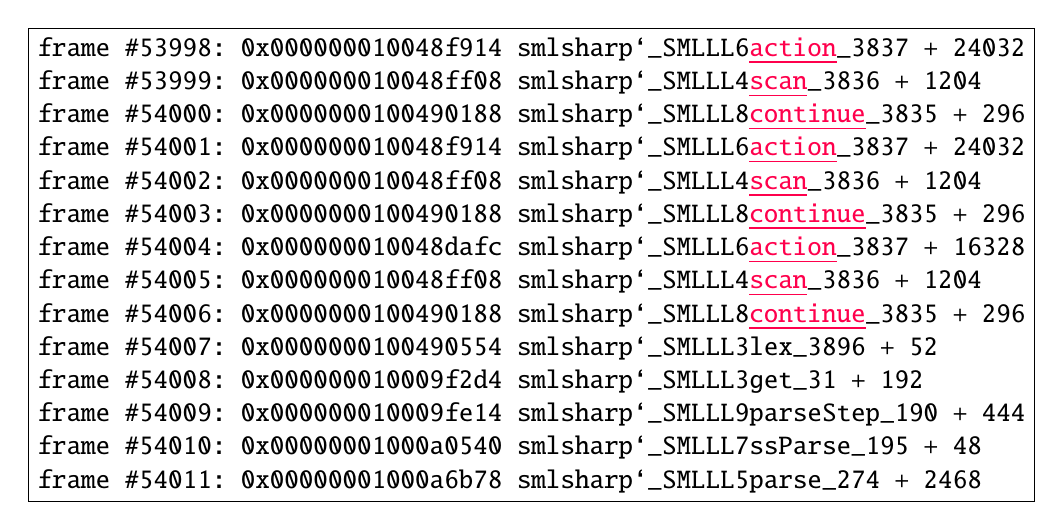
\begin{tikzpicture}
\node[draw,align=left] at (0,0) {%
\code{frame \#53998: 0x000000010048f914 smlsharp`\_SMLLL6\focus{action}\_3837 + 24032}\\
\code{frame \#53999: 0x000000010048ff08 smlsharp`\_SMLLL4\focus{scan}\_3836 + 1204}\\
\code{frame \#54000: 0x0000000100490188 smlsharp`\_SMLLL8\focus{continue}\_3835 + 296}\\
\code{frame \#54001: 0x000000010048f914 smlsharp`\_SMLLL6\focus{action}\_3837 + 24032}\\
\code{frame \#54002: 0x000000010048ff08 smlsharp`\_SMLLL4\focus{scan}\_3836 + 1204}\\
\code{frame \#54003: 0x0000000100490188 smlsharp`\_SMLLL8\focus{continue}\_3835 + 296}\\
\code{frame \#54004: 0x000000010048dafc smlsharp`\_SMLLL6\focus{action}\_3837 + 16328}\\
\code{frame \#54005: 0x000000010048ff08 smlsharp`\_SMLLL4\focus{scan}\_3836 + 1204}\\
\code{frame \#54006: 0x0000000100490188 smlsharp`\_SMLLL8\focus{continue}\_3835 + 296}\\
\code{frame \#54007: 0x0000000100490554 smlsharp`\_SMLLL3lex\_3896 + 52}\\
\code{frame \#54008: 0x000000010009f2d4 smlsharp`\_SMLLL3get\_31 + 192}\\
\code{frame \#54009: 0x000000010009fe14 smlsharp`\_SMLLL9parseStep\_190 + 444}\\
\code{frame \#54010: 0x00000001000a0540 smlsharp`\_SMLLL7ssParse\_195 + 48}\\
\code{frame \#54011: 0x00000001000a6b78 smlsharp`\_SMLLL5parse\_274 + 2468}%
};
\end{tikzpicture}
\end{center}

\end{frame}

\begin{frame}{スタック溢れを起こしたコード(iml.lex.sml)}
\begin{prog}
fun \focus{continue} () =\\
~~~~let\\
~~~~~~fun \focus{scan} ($\cdots$) =\\
~~~~~~~~~~let\\
~~~~~~~~~~~~fun \focus{action} ($\cdots$) =\\
~~~~~~~~~~~~~~~~case $\cdots$ o\=f $\cdots$ => \focus{action} ($\cdots$)\\
                               \>| $\cdots$ => \focus{continue} ()\\
                               \>| $\cdots$ => result\\
~~~~~~~~~~in case $\cdots$ o\=f $\cdots$ => \focus{action} ($\cdots$)\\
                            \>| $\cdots$ => \focus{scan} ($\cdots$)\\
                            \>| $\cdots$ => result\\
~~~~~~~~~~end\\
~~~~in \focus{scan} ($\cdots$)\\
~~~~end
\end{prog}

\only<2->{
\begin{textblock}{120}(108,10)
\begin{tikzpicture}
\draw[white] (-2,-5) rectangle ++(4.5,7);
\node (E) at (0,1.5) {entry};
\node[draw,fill=white,rounded corners=6pt,minimum width=60pt] (C) at (0,0) {\code{continue}};
\only<3->{\node[draw,fill=white,rounded corners=6pt,minimum width=60pt] (S) at (0,-1.5) {\code{scan}};}
\only<4->{\node[draw,fill=white,rounded corners=6pt,minimum width=60pt] (A) at (0,-3) {\code{action}};}
\only<6->{\node (R) at (0,-4.5) {exit};}
\draw[thick,-latex] (E) -- (C);
\only<3->{\draw[thick,-latex] (C) -- (S);}
\only<4->{\draw[thick,-latex] (S) -- (A);}
\only<5->{\draw[thick,-latex] (S) to[out=345,in=15,looseness=4] (S);}
\only<7->{\draw[thick,-latex] (A) to[out=345,in=15,looseness=3] (A);}
\only<8->{\draw[thick,-latex] (A) to[out=330,in=30,looseness=2] (C);}
\only<6->{\draw[thick,-latex] (S) to[out=200,in=160] (R);}
\only<9->{\draw[thick,-latex] (A) -- (R);}
\end{tikzpicture}
\end{textblock}
}

\end{frame}

\begin{frame}{どうしよう…}

CPS変換して全ての関数適用を末尾呼び出しにすれば?
\begin{itemize}
\item Cと同じ実行モデルを指向する\smlsharp{}でそれはちょっと…
\end{itemize}

\bigskip

ジャンプを意図してそうな末尾呼び出しは全部本物のジャンプにせねばなるまい
\begin{itemize}
\item 再帰呼び出しは関数を越える
\begin{itemize}
\item このネストした相互再帰関数群から二重ループを作れるか…?
\end{itemize}
\item コンパイル単位内を跨ぐ場合は諦めてもいい
\begin{itemize}
\item 逆にコンパイル単位内なら徹底的にやりたい
\end{itemize}
\item 末尾位置の特定はアンカリー化とも絡む
\begin{itemize}
\item アンカリー化も同時にやらざるを得ない
\end{itemize}
\end{itemize}

\end{frame}

\begin{frame}{基本的な方針}

関数$A$が関数$B$を末尾呼び出し(カリー化されている場合を含む)しているとき,
$B$が(自己末尾再帰を除いて)$A$からしか呼ばれないならば,$B$を$A$に統合し,
末尾呼び出しをジャンプに置き換える.これをできなくなるまで繰り返す.

\begin{center}
\begin{tikzpicture}
\draw[white] (-3,-3.5) rectangle ++(6,5.3);
\node (E) at (0,1.4) {外部};
\node[alt=<2->{}{draw},fill=white,rounded corners=6pt,minimum width=60pt] (C) at (0,0) {\code{continue}};
\node[alt=<2->{}{draw},fill=white,rounded corners=6pt,minimum width=60pt] (S) at (0,-1.4) {\code{scan}};
\node[alt=<3->{}{draw},fill=white,rounded corners=6pt,minimum width=60pt] (A) at (0,-2.8) {\code{action}};
\draw[thick,-latex,dashed] (E) -- (C);
\draw[thick,-latex] (C) -- (S);
\draw[thick,-latex] (S) -- (A);
\draw[thick,-latex] (S) to[out=345,in=15,looseness=4] (S);
\draw[thick,-latex] (A) to[out=345,in=15,looseness=3] (A);
\draw[thick,-latex] (A) to[out=330,in=30,looseness=2] (C);
\only<2>{\draw[rounded corners=6pt] (-1.6,-1.8) rectangle ++(3.2,2.1);}
\only<3>{\draw[rounded corners=6pt] (-1.6,-3.3) rectangle ++(3.2,3.6);}

\end{tikzpicture}
\end{center}

\end{frame}

\begin{frame}{ジャンプを関数適用以外でどう表現するか?}

\smlsharp{}では中間言語に「関数を越えない例外機構」を導入.
\begin{itemize}
\item \code{throw}すると式のネストを飛び越えて\code{catch}にジャンプ
\item \code{catch}内での\code{throw}を許すことでバックエッジを表現
\end{itemize}

\begin{center}
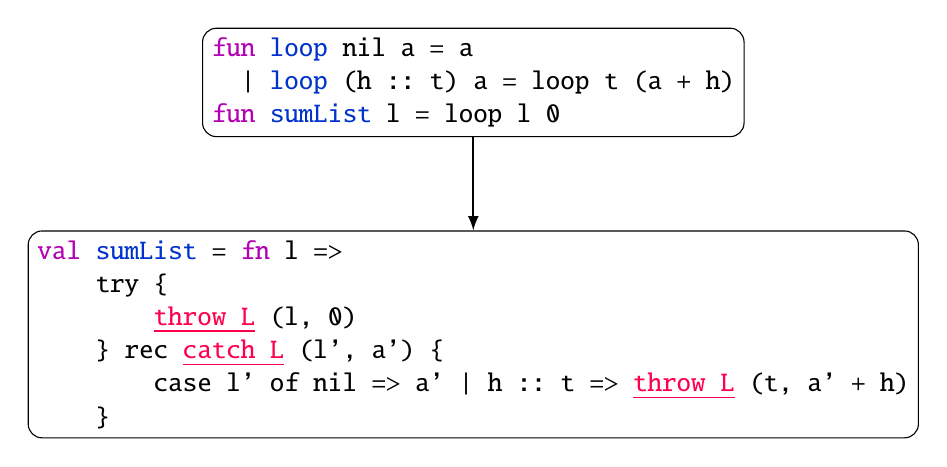
\begin{tikzpicture}
\node[draw,align=left,rounded corners=5pt] (S) at (0,0){%
\code{\KW{fun} \ID{loop} nil a = a}\\
\code{~~| \ID{loop} (h :: t) a = loop t (a + h)}\\
\code{\KW{fun} \ID{sumList} l = loop l 0}};
\node[draw,align=left,rounded corners=5pt] (I) at (0,-3.2){%
\code{\KW{val} \ID{sumList} = \KW{fn} l =>}\\
\code{~~~~try \{}\\
\code{~~~~~~~~\focus{throw L} (l, 0)}\\
\code{~~~~\} rec \focus{catch L} (l', a') \{}\\
\code{~~~~~~~~case l' of nil => a' | h :: t => \focus{throw L} (t, a' + h)}\\
\code{~~~~\}}};
\draw[thick,-latex] (S) -- (I);
\end{tikzpicture}
\end{center}

\end{frame}

\begin{frame}{末尾呼び出しコンパイル(TailCallCompile)}

この問題に対してやれることを力技で全部やる!

\begin{enumerate}
\item ステップ0:全ての変数を名前替えしてユニークな識別子を振る
\item ステップ1:関数間呼び出し関係の抽出と整理
\item ステップ2:コールグラフの作成とクラスタリング
\item ステップ3:これまでに得た解析結果に基づいてコード変換
\end{enumerate}

\bigskip
{\footnotesize (調べるより先に手を動かしたい(←悪い癖))}

\end{frame}

\begin{frame}{ステップ1-1: 呼び出し関係解析}

解析結果を蓄える集合を$R$とする.
\begin{enumerate}
\item 関数定義\code{val $f$ = fn $y_1$ => $\cdots$ => fn $y_m$ => $e$}を
見つけたら
\[[\code{$f$ is fun($y_1\cdots y_m$)}]\]
を$R$に追加.
\medskip
\item 関数$f$の中に関数適用式$g\ e_1\ \cdots\ e_n$($n \ge 0$)を見つけたら
\[[\code{$f$ calls $g(e_1\cdots e_n)$ at $p$}]\]
を$R$に追加.
\begin{itemize}
\item $p$(\code{mid}または\code{tail})は末尾位置かそうでないかを表すフラグ
\item トップレベルは$\mathit{Top}$という特別な関数名を持つとする
\item 関数$f$内の無名関数は\code{$f$?}という名前を持つとする
\end{itemize}
\end{enumerate}

\end{frame}

\begin{frame}{ステップ1-2: デッドコード除去}

以下の条件をすべて満たす最小の$L$を求める.
\begin{enumerate}
\item $\mathit{Top} \in L$
\item $[\code{$f$ calls $g(e_1\cdots e_n)$ at $p$}] \in R$かつ$f \in L$ならば
$g\in L$
\item $[\code{$f$? calls $g(e_1\cdots e_n)$ at $p$}] \in R$かつ$f \in L$ならば
$g\in L$
\end{enumerate}

\bigskip
$[\code{$f$ calls $g(e_1\cdots e_n)$ at $p$}] \in R$それぞれについて
\begin{itemize}
\item $f\not\in L$または$g\not\in L$ならば$R$から削除
\end{itemize}

\end{frame}

\begin{frame}{ステップ1-3: callerとcalleeで引数の最大数を揃える}

\only<1>{
例えば$[\code{f is fun($y_1y_2y_3$)}]$に対して
\begin{itemize}
\item $[\code{g calls f$(e_1e_2)$ at $p_1$}]$
\item $[\code{h calls f$(e_1)$ at $p_2$}]$
\end{itemize}
のように3未満の引数でしか呼ばれていないとき,\code{f}を2引数関数に読み替える.
\begin{center}
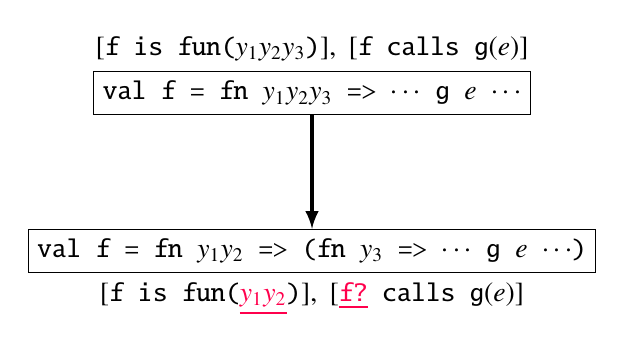
\begin{tikzpicture}
\node[draw,label=above:{$[\code{f is fun($y_1y_2y_3$)}],\;[\code{f calls g$(e)$}]$}] (B) at (0,2){\code{val f = fn $y_1y_2y_3$ => $\cdots$ g $e$ $\cdots$}};
\node[draw,label=below:{$[\code{f is fun(\focus{$y_1y_2$})}],\;[\code{\focus{f?} calls g$(e)$}]$}] (A) at (0,0){\code{val f = fn $y_1y_2$ => (fn $y_3$ => $\cdots$ g $e$ $\cdots$)}};
\draw[very thick,-latex] (B) -- (A);
\end{tikzpicture}
\end{center}
}
\only<2>{
逆に$[\code{f is fun($y_1y_2y_3$)}]$に対して
\begin{itemize}
\item $[\code{g calls f$(e_1e_2e_3e_4)$ at $p_1$}]$
\item $[\code{h calls f$(e_1e_2)$ at $p_2$}]$
\end{itemize}
のように3より多い引数で呼ばれている場合があるとき,超過分の引数を削除する.
\begin{center}
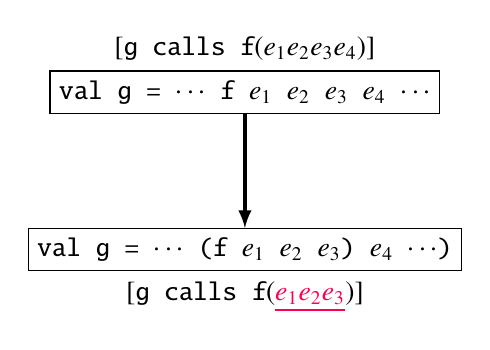
\begin{tikzpicture}
\node[draw,label=above:{$[\code{g calls f$(e_1e_2e_3e_4)$}]$}] (B) at (0,2){\code{val g = $\cdots$ f $e_1\ e_2\ e_3\ e_4$ $\cdots$}};
\node[draw,label=below:{$[\code{g calls f$(\focus{e_1e_2e_3})$}]$}] (A) at (0,0){\code{val g = $\cdots$ (f $e_1\ e_2\ e_3$) $e_4$ $\cdots$)}};
\draw[very thick,-latex] (B) -- (A);
\end{tikzpicture}
\end{center}
}
\end{frame}

\begin{frame}{ステップ1-4: eta-expansion}

例えば$[\code{f is fun($y_1y_2y_3$)}]$に対して
\begin{itemize}
\item $[\code{g calls f$(e_1e_2)$ at $p$}]$
\end{itemize}
のように3未満の引数で呼ばれている場合があるとき,
\[\code{val f$_2$ = fn $y_1y_2$ => (fn $y_3$ => f $y_1y_2y_3$)}\]
のような関数定義をあとで挿入することにして,以下の情報を$R$に追加する.
\begin{itemize}
\item $[\code{f$_2$ is fun($y_1y_2$)}]$
\item $[\code{f$_2$? calls f$(y_1y_2y_3)$ at tail}]$
\item $[\code{f$_2$ is eta(f, $2$)}]$
\end{itemize}

\medskip

さらに$[\code{g calls f$(e_1e_2)$ at $p$}]$を$[\code{g calls f$_2(e_1e_2)$ at $p$}]$に置き換える.

\end{frame}

\begin{frame}{ステップ2-1: コールグラフの作成}

関数名を頂点,末尾呼び出しを辺とする有向グラフを構築する.
\begin{enumerate}
\item $[\code{$f$ is fun($\cdots$)}] \in R$ならば$f$を頂点としてグラフに加える
\item $[\code{$g$ calls $f(\cdots)$ at tail}] \in R$ならば
$g$から$f$への辺をグラフに加える
\end{enumerate}

\bigskip

さらに,以下の条件を満たす頂点$f$を「入口頂点」と呼ぶことにする:
\begin{enumerate}
\item[] ある$g$が存在し$[\code{$g$ calls $f(\cdots)$ at mid}] \in R$
\end{enumerate}

\end{frame}

\begin{frame}{ステップ2-2: グラフ彩色}

入口頂点$f$それぞれについて,$f$から到達可能なすべての頂点$g$に色$f$を塗る.

\bigskip

2つ以上の色が塗られた頂点$g$があれば,$g$に入る全ての辺を削除し,
$g$を入口頂点に加えて,彩色を最初からやり直す.

\bigskip

彩色が終わったら,
$[\code{$f$ calls $g(\cdots)$ at tail}]\in R$それぞれについて,
\begin{itemize}
\item $f$と$g$の色が同じでなければ
$[\code{$f$ calls $g(\cdots)$ at mid}]$に置き換える
\end{itemize}

\bigskip

ここまでで,統合すべき関数の集合が定まった.

(同じ色を持つ関数は同じ関数の一部となる)

\end{frame}

\begin{frame}{ステップ2-3: 引数伝播}

ある仮引数に必ず特定の実引数が渡されることが静的に読み切れるならば,
その仮引数の参照をその特定の値に置き換えたい.

\bigskip

項集合に$\top$(静的には不明)と$\bot$(未使用)を加えて束を作り,
仮引数に関する連立不等式を立て,その最小解をunion-findで求める.

\medskip

\begin{tabbing}
$[\code{$f$ is fun($y_1\cdots y_n$)}] \in R$それぞれについて:\\
\qquad
$g$の色が$g$ならば,連立不等式に$y_1\ge y_1, \ldots, y_n\ge y_n$を加える\\
\qquad
$[\code{$g$ calls $f(e_1\cdots e_n)$ at tail}] \in R$それぞれについて:\\
\qquad\qquad
連立不等式に$y_1\ge e_1, \ldots, y_n\ge e_n$を加える
\end{tabbing}

\end{frame}

\begin{frame}{ステップ3: 関数定義の変換}

関数定義\code{val $f$ = fn $y_1$ => $\cdots$ => fn $y_m$ => $e$}それぞれについて:
\begin{tabbing}
\qquad
誰からも呼ばれていない($[\code{$g$ calls $f(\cdots)$ at $p$}] \not\in R$)
ならば削除.\\
\qquad
$[\code{$f$ is fun($y_1\cdots y_M$)}] \in R$のはずなので,
$M$個の引数でアンカリー化.\\
\qquad
$[\code{$f_i$ is eta($f, i$)}] \in R$それぞれについて関数定義を生成.\\
\qquad
$f$の色が$f$ならば:\\
\qquad\qquad
$[\code{$g$ calls $f(\cdots)$ at mid}] \in R$がただひとつだけ存在するならば\\
\qquad\qquad\qquad
インライン展開のために記憶して削除.\\
\qquad\qquad
そうでなければ,関数定義をこの場にそのまま残す.\\
\qquad
$[\code{$g$ calls $f(\cdots)$ at $p$}] \in R$がただひとつだけ存在するならば\\
\qquad\qquad
インライン展開のために記憶して削除.\\
\qquad
この関数定義を含む関数の色と$f$の色が同じなら\\
\qquad\qquad
この場で\code{catch}に変換.\\
\qquad
以上のいずれにも当てはまらなければ\\
\qquad\qquad
\code{catch}化のために記憶して削除.
\end{tabbing}

\end{frame}

\begin{frame}{ステップ3: 関数適用式の変換}

関数適用式\code{$f$ $e_1\ \cdots\ e_n$}それぞれについて:
\begin{tabbing}
\qquad $[\code{$f$ is fun($y_1\cdots y_m$)}] \in R$のはず.\\
\qquad $n < m$ならば,
$[\code{$f_n$ is eta($f, n$)}] \in R$のはずなので,$f$を$f_n$に置き換える.\\
\qquad $\mathrm{min}(n, m)$でアンカリー化.\\
\qquad $f$がインライン関数として記憶されているならば\\
\qquad\qquad この位置で$f$をインライン展開\\
\qquad 末尾位置でありかつこの関数適用を含む関数の色と$f$の色が同じならば\\
\qquad\qquad \code{throw}に変換\\
\qquad そうでなければ,関数適用をここに残す.
\end{tabbing}

\end{frame}

\begin{frame}{末尾呼び出しコンパイルフェーズの実装}

\begin{itemize}
\item 全部で1456行:\url{https://github.com/smlsharp/smlsharp/tree/master/src/compiler/compilePhases/tailcallcompile/main}
\item 関数型の皮をかぶった手続き的コード
\begin{itemize}
\item 関数型言語でも手続き的に書けるし書くべきときもある
\end{itemize}
\item 多相関数(型抽象)にも対応(「色=関数名+型インスタンス」と取る)
\end{itemize}

\end{frame}

\PART{部分評価に基づくコードの最適化}

\begin{frame}{純粋な速さの追求:関数を関数でなくす}

関数型言語では関数が計算手続きを書き表す中核となるため,
多量の関数抽象と関数適用がプログラム中に現れる.しかし:
\begin{itemize}
\item 関数抽象(クロージャ)は一般にはメモリ確保を伴う
\item 関数適用(コール)は一般にはスタックフレーム確保を伴う
\end{itemize}
操作であり,安直に実装すると,遅い.

\bigskip

実行効率のためには,如何にこれらをこのとおりに実装「しない」かが重要.

\begin{itemize}
\item 先ほどの末尾呼び出しコンパイルもこの手の方向性を共有
\end{itemize}

\end{frame}

\begin{frame}{実行前に消せる関数適用は全部消しておきたい}

\begin{prog}
\KW{fun} \ID{score} x y = x * 2 + y * 3\\
\KW{fun} \ID{left} x = score x 4\\
\KW{fun} \ID{right} y = score 4 y
\end{prog}
みたいなコードがあったとき,
\begin{prog}
score x 4 $\longrightarrow$ x * 2 + 4 * 3 $\longrightarrow$ x * 2 + 12\\
score 4 y $\longrightarrow$ 4 * 2 + y * 3 $\longrightarrow$ 8 + y * 3
\end{prog}
なわけだから結局
\begin{prog}
\KW{fun} \ID{left} x = x * 2 + 12\\
\KW{fun} \ID{right} x = 8 + y * 3
\end{prog}
だよね,と実行前に見切っておきたい.

\end{frame}

\begin{frame}{部分評価}

あるプログラム(関数)の入力(引数)の一部が静的に定まっているとき,
その入力をあらかじめ与えて特化したプログラムを生成する技法.

\bigskip

例:
\begin{prog}
~~~~\KW{fun} \ID{score} x y = x * 2 + y * 3
\end{prog}
に対して$\code{x} = 4$であることがあらかじめわかっているとき,
$\code{x} = 4$が関わる計算を全て事前に行って特化した
\begin{prog}
~~~~\KW{fun} \ID{score4} y = 8 + y * 3
\end{prog}
を実行前に作り出す.

\end{frame}

\begin{frame}{部分評価による最適化の可能性}

ソースプログラム中に含まれる静的な情報に対して,
コンパイル単位内の全ての関数を実行前に特化しておきたい.

\bigskip

インライン展開や定数伝播をする最適化器はすでにある(TCOptimization)
\begin{itemize}
\item インライン展開はするが評価まではしてくれない
\item 評価順序が変わってしまうからβ簡約はしない(\code{let}を挿入)
\item 再帰関数は展開しない
\item 性能に満足できない
\end{itemize}

\bigskip

コンパイラにインタプリタを内蔵すればよいのではないか
\begin{itemize}
\item MLインタプリタはふつう自然意味論に基づいて書くよね
\item 部分評価器を自然意味論のように書けたら嬉しい
\item (関連研究調べる前にとりあえず手を動かしたい…)
\end{itemize}

\end{frame}

\begin{frame}{自然意味論(natural semantics)}

プログラム$M$の意味を,
環境$E$の下で$M$は値$v$に評価される,
という判定を導出する規則の積み重ねによって与える意味論.
ほぼインタプリタそのもの.

\begin{tabbing}
\qquad\infer{}{$E\{x\mapsto v\} \vdash x \Downarrow v$}
\\[10pt]
\qquad\infer{}{$E \vdash \lambda x. M \Downarrow \mathrm{Cls}(E,x,M)$}
\\[18pt]
\qquad\infer
{$E \vdash M_1 \Downarrow \mathrm{Cls}(E',x,M)$\qquad
 $E \vdash M_2 \Downarrow v_2$\qquad
 $E'\{x\mapsto v_2\} \vdash M \Downarrow v$}
{$E \vdash M_1\ M_2 \Downarrow v$}
\end{tabbing}

\bigskip

「横線の上にある判定が全て得られたならば下の判定が得られる」と読む.

\medskip

式全体を値に移してしまうため残余プログラムは得られない….

\end{frame}

\begin{frame}{部分評価のための自然意味論}

残余プログラムを保存するための場所(ヒープ)を用意しよう.

\begin{itemize}
\item ヒープには「将来使うデータ」や「今は行わない計算」を置くことができる
\item 「未知の値」も,ヒープに置いたことにして,
(実体を参照できない)ポインタとして表現できるのでは
\item 実行順序を保存するためポインタにはヒープ内で順序を与える
\item 「今は行わない計算」はポインタやヒープ内順序を介して
ヒープ内でグラフ構造をなすはず.これは残余プログラムそのもの
\end{itemize}

\end{frame}

\begin{frame}{部分評価のための自然意味論:評価判定のスケッチ}

\begin{center}\large
$H, E \vdash M \Rightarrow H', v$
\end{center}
\begin{itemize}
\item $H$(ヒープ):「今は行わない計算」を保持するグローバルな記憶装置.
\item $E$(変数環境):変数への既知の値の対応付け.
\item $M$(プログラム):部分評価対象のプログラム.
\item $H'$(ヒープ差分):グローバルなヒープに新たに加えられるデータ列.
\item $v$(値):評価結果の値.定数$c$かポインタ$p$のいずれか.
\end{itemize}

\bigskip

ヒープ$H$と環境$E$の下でプログラム$M$を評価すると,
ヒープには新たに$H'$が割り付けられ,その結果として値$v$が得られる.

\end{frame}

\begin{frame}{部分評価器のための自然意味論:評価規則のスケッチ(1)}

定数式,変数式は,その値を返すだけ.

\begin{tabbing}
\infer{}{$H, E \vdash c \Rightarrow [], c$}
\\[5pt]
\infer{}{$H, E \vdash p \Rightarrow [], p$}
\\[5pt]
\infer{}{$H, E\{x\mapsto v\} \vdash x \Rightarrow [], v$}
\end{tabbing}

\end{frame}

\begin{frame}{部分評価器のための自然意味論:評価規則のスケッチ(2)}

\begin{center}
\infer
{$H, E\{x\mapsto p\} \vdash M \Rightarrow H', v$}
{$H, E \vdash \lambda x. M \Rightarrow [p'\mapsto \lambda x. [p\mapsto x](\langle H'; v \rangle)], p'$}
($p$, $p'$ fresh)
\end{center}

\begin{itemize}
\item 仮引数に「未知の値」(何も指さないポインタで表現)を入れて本体を評価する
\item 本体を評価したらヒープ差分$H'$が得られる.
この$H'$には$M$の残余プログラムが保存されている.
\item $\langle H'; v\rangle$は「$H'$にしまわれている計算を
$v$に至る範囲で再生する」ような式を作る演算(いわゆるlet-insertion)
\item 生成された関数抽象はヒープに割り付けて,そのポインタを評価結果の値とする.
\end{itemize}

\end{frame}

\begin{frame}{部分評価器のための自然意味論:評価規則のスケッチ(3)}

\begin{center}
\infer
{$H, E \vdash M_1 \Rightarrow H_1, v_1$\qquad
 $HH_1, E \vdash M_2 \Rightarrow H_2, v_2$\qquad
 $HH_1H_2(v_1) = \lambda x.M$\\
 $HH_1H_2, \{x\mapsto v_2\} \vdash M \Rightarrow H_3, v$}
{$H, E \vdash M_1\ M_2 \Rightarrow H_1H_2H_3, v$}
\end{center}
\begin{itemize}
\item $M_1$と$M_2$をそれぞれこの順に評価する.
\item グローバルなヒープにはヒープ差分が蓄積されていく.
\item ポインタ$v_1$を参照してヒープからオブジェクトを取り出す.
\item それが関数抽象ならば,実引数を渡して関数本体を評価する.
\item ヒープにしまわれていた関数抽象は自由変数を持たない(すでに評価されて
定数になっている).
\end{itemize}

\end{frame}

\begin{frame}{部分評価器のための自然意味論:評価規則のスケッチ(4)}

\begin{center}
\infer
{$H, E \vdash M_1 \Rightarrow H_1, v_1$\qquad
 $HH_1, E \vdash M_2 \Rightarrow H_2, v_2$\qquad
 $HH_1H_2(v_1) \not= \lambda x.M$}
{$H, E \vdash M_1\ M_2 \Rightarrow H_1H_2[p\mapsto v_1\ v_2], p$}
($p$ fresh)
\end{center}
\begin{itemize}
\item $M_1$と$M_2$をそれぞれこの順に評価する.グローバルなヒープには
評価結果のヒープ差分が蓄積されていく.
\item ポインタ$v_1$を参照してヒープからオブジェクトを取り出す.
\item それが関数抽象でない(参照できない場合も含む)ならば,
この関数適用は「今は行えない」ので,
「関数適用$v_1\ v_2$を計算すること」をヒープにしまう.
\item ヒープにしまった計算へのポインタを評価結果とする.
\end{itemize}

\end{frame}

\begin{frame}{評価例}

\begin{tikzpicture}[y=18pt]
\draw[white] (0,-.5) rectangle (10,10.5);

\node[anchor=west] (S) at (0,0){
$\alt<2->{}{\phantom}{[], \emptyset \vdash\;} (\lambda x. \lambda y. (x + (1 + 2)) + y)\ 3 \alt<2->{}{\phantom}{\;\Rightarrow\;}
\alt<28->{}{\phantom}{[p_6\mapsto \lambda x.\lambda y.(x+3)+y,
                       p_9\mapsto \lambda y.(6 + y)], p_9}$
};
\only<2->{\draw (S.north west) -- (S.north east);}

\only<19->{
\node[anchor=west] (S3) at (0,1){
$[p_6\mapsto \lambda x.\lambda y.(x+3)+y], \{x\mapsto 3\} \vdash \lambda y.(x+3)+y \Rightarrow\;
\alt<27->{}{\phantom}{[p_9\mapsto \lambda y.(6 + y)], p_9}$
};}
\only<21->{
\draw (S3.north west) -- (S3.north east);
\node[anchor=west] (S31) at (0,2){
$[p_6\mapsto \lambda x.\lambda y.(x+3)+y], \{x\mapsto 3,y\mapsto p_7\} \vdash (x+3)+y \Rightarrow\;
\alt<26->{}{\phantom}{[p_8\mapsto 6 + p_7], p_8}$
};}
\only<22->{
\draw (S31.north west) -- (S31.north east);
\node[anchor=west] (S31) at (0,4){
$[p_6\mapsto \lambda x.\lambda y.(x+3)+y], \{x\mapsto 3,y\mapsto p_7\} \vdash x+3 \Rightarrow\;
\alt<23->{}{\phantom}{[], 6}$
};}
\only<24->{
\node[anchor=west] (S31) at (0,3){
$[p_6\mapsto \lambda x.\lambda y.(x+3)+y], \{x\mapsto 3,y\mapsto p_7\} \vdash y \Rightarrow\;
\alt<25->{}{\phantom}{[], p_7}$
};}

\only<17-19>{
\node[anchor=west] (S2) at (0,2){
$[p_6\mapsto \lambda x.\lambda y.(x+3)+y], \emptyset \vdash 3 \Rightarrow\;
\alt<18->{}{\phantom}{[], 3}$
};}
\only<3-19>{
\node[anchor=west] (S1) at (0,3){
$[], \emptyset \vdash \lambda x. \lambda y. (x + (1 + 2)) + y \Rightarrow\;
\alt<16->{}{\phantom}{[p_6\mapsto \lambda x.\lambda y.(x + 3) + y], p_6}$
};}
\only<4-16>{
\draw (S1.north west) -- (S1.north east);
\node[anchor=west] (S11) at (0,4){
$[], \{x\mapsto p_1\} \vdash \lambda y. (x + (1 + 2)) + y \Rightarrow\;
\alt<15->{}{\phantom}{[p_5\mapsto \lambda y. (p_1 + 3) + y], p_5}$
};}
\only<5-16>{
\draw (S11.north west) -- (S11.north east);
\node[anchor=west] (S111) at (0,5){
$[], \{x\mapsto p_1,y\mapsto p_2\} \vdash (x + (1 + 2)) + y \Rightarrow\;
\alt<14->{}{\phantom}{[p_3\mapsto p_1+3, p_4\mapsto p_3 + p_2], p_4}$
};}
\only<12-16>{
\node[anchor=west] (S112) at (0,6){
$[p_3\mapsto p_1 +3], \{x\mapsto p_1,y\mapsto p_2\} \vdash y \Rightarrow
\alt<13->{}{\phantom}{[], p_2}$
};}
\only<6-16>{
\draw (S111.north west) -- (S111.north east);
\node[anchor=west] (S1111) at (0,7){
$[], \{x\mapsto p_1,y\mapsto p_2\} \vdash x + (1 + 2) \Rightarrow\;
\alt<11->{}{\phantom}{[p_3\mapsto p_1 + 3], p_3}$
};}
\only<7-11>{
\draw (S1111.north west) -- (S1111.north east);
\node[anchor=west] (S11111) at (0,9){
$[], \{x\mapsto p_1,y\mapsto p_2\} \vdash x \Rightarrow
\alt<8->{}{\phantom}{[], p_1}$
};}
\only<9-11>{
\draw (S1111.north west) -- (S1111.north east);
\node[anchor=west] (S11111) at (0,8){
$[], \{x\mapsto p_1,y\mapsto p_2\} \vdash 1 + 2 \Rightarrow
\alt<10->{}{\phantom}{[], 3}$
};}

\end{tikzpicture}
\end{frame}

\begin{frame}{従来の自然意味論との違い}

\begin{itemize}
\item ヒープの存在
\begin{itemize}
\item とはいえヒープを持たないインタプリタはないので不自然ではない
\end{itemize}
\bigskip
\item 「未知の値」もポインタにすることで
どんなプログラムもとりあえず評価できる.
関数本体も呼び出し前に評価してしまう
\begin{itemize}
\item 不正な状態($\mathit{Wrong}$)にならない.プログラムが止まるなら
必ず正当な値が得られる.$\mathit{Wrong}$を導くはずだった誤った計算は
「今はできない・やらない」のでヒープにしまわれる.
\end{itemize}
\bigskip
\item ポインタとポインタ順序を再帰的に辿ることで残余プログラムが得られる
\begin{itemize}
\item 関数適用の回数と順序を保存しなければならないことに気を付ける.
\end{itemize}
\end{itemize}

\end{frame}

\begin{frame}{フルスケールの\smlsharp{}へのスケールアップ}

「ヒープがある」のでポインタ操作を明示する必要があることさえ
わかっていれば,インタプリタをさくさく書ける.
\bigskip
\begin{itemize}
\item 部分評価器のコアの実装は1028行:\url{https://github.com/smlsharp/smlsharp/tree/master/src/compiler/compilePhases/partialevaluation/main}
\begin{itemize}
\item TCOptimizationは1417行
\end{itemize}
\bigskip
\item 部分評価をどこまでやるかは実装者の裁量
\begin{itemize}
\item 大きな関数の適用はやらない
\item 相互再帰関数間で相互再帰の相手を展開する
\end{itemize}
\end{itemize}

\end{frame}

\PART{評価とまとめ}

\begin{frame}{結局\smlsharp{}はどれだけ速くなったか}

比較対象:
\begin{enumerate}
\item[(A)] \smlsharp{} 4.1.0でコンパイルした\smlsharp{} 4.2.0
\item[(B)] \smlsharp{} 4.2.0でコンパイルした\smlsharp{} 4.2.0
\end{enumerate}

\bigskip

計測対象:
\begin{itemize}
\item \smlsharp{} 4.2.0のMatchCompiler.smlのコンパイルにかかるuser time
\item 10回測って平均を求める
\end{itemize}

\bigskip

計測環境:
\begin{itemize}
\item AMD EPYC 7501 2.0GHz, 128 GB RAM, NixOS unstable (2025-06-13)
\item LLVM 19.1.7
\end{itemize}

\bigskip

結果:
\begin{enumerate}
\item[(A)] 4.919秒
\item[(B)] 3.270秒 \focus{(-33.5\%)}

%time SMLSHARP_HEAPSIZE=32M:2G src/compiler/smlsharp -Bsrc -S -o /dev/null ~/work/smlsharp-4.2.0/src/compiler/compilePhases/matchcompilation/main/MatchCompiler.sml
%(A)
%user	0m4.946s
%user	0m4.934s
%user	0m4.901s
%user	0m4.895s
%user	0m4.915s
%user	0m4.917s
%user	0m4.937s
%user	0m4.905s
%user	0m4.932s
%user	0m4.903s
%(B)
%user	0m3.260s
%user	0m3.272s
%user	0m3.256s
%user	0m3.280s
%user	0m3.273s
%user	0m3.263s
%user	0m3.283s
%user	0m3.277s
%user	0m3.278s
%user	0m3.262s

\end{enumerate}

\end{frame}

\begin{frame}{各最適化はどれだけ効いているか}
\def\CHK{\tikz\fill[scale=0.4](0,.35) -- (.25,0) -- (1,.7) -- (.25,.15) -- cycle;}

\smlsharp{} 4.2.0で最適化オプションを変えてコンパイルした\smlsharp{} 4.2.0でMatchCompiler.smlをコンパイルするのにかかったuser time

\begin{center}
\begin{tabular}{|c|c|c|c|c|l}\cline{1-5}
TailCallComp & UncurryOpt & PartEval & TCOpt & 測定結果 & \phantom{(-00.0\%)}\\\cline{1-5}
             &            &          &       & 6.527秒 & \only<2>{←基準}\\\cline{1-5}
    \CHK     &            &          &       & 3.716秒 & \only<2>{\focus{(-43.1\%)}}\only<3>{\focus{(-28.1\%)}}\only<4>{←基準}\\\cline{1-5}
    \CHK     &            &   \CHK   &       & 3.264秒 & \only<4>{\focus{(-15.2\%)}}\\\cline{1-5}
    \CHK     &            &          & \CHK  & 3.713秒 & \only<4>{(-\phantom{0}0.1\%)}\\\cline{1-5}
             &    \CHK    &          &       & 5.171秒 & \only<2>{(-20.8\%)}\only<3,4>{←基準}\\\cline{1-5}
             &    \CHK    &   \CHK   &       & 4.385秒 & \only<4>{\focus{(-12.2\%)}}\\\cline{1-5}
             &    \CHK    &          & \CHK  & 4.649秒 & \only<4>{(-10.1\%)}\\\cline{1-5}
\end{tabular}
\end{center}

%(NONE)
%user	0m6.535s
%user	0m6.535s
%user	0m6.568s
%user	0m6.525s
%user	0m6.520s
%user	0m6.503s
%user	0m6.522s
%user	0m6.523s
%user	0m6.541s
%user	0m6.500s
%(TCC)
%user	0m3.716s
%user	0m3.721s
%user	0m3.717s
%user	0m3.729s
%user	0m3.715s
%user	0m3.728s
%user	0m3.700s
%user	0m3.707s
%user	0m3.720s
%user	0m3.704s
%(UO)
%user	0m5.156s
%user	0m5.166s
%user	0m5.168s
%user	0m5.183s
%user	0m5.166s
%user	0m5.160s
%user	0m5.155s
%user	0m5.189s
%user	0m5.193s
%user	0m5.172s
%(UO+PE)
%user	0m4.385s
%user	0m4.384s
%user	0m4.396s
%user	0m4.397s
%user	0m4.393s
%user	0m4.382s
%user	0m4.374s
%user	0m4.382s
%user	0m4.369s
%user	0m4.391s
%(TCC+PE)
%user	0m3.282s
%user	0m3.257s
%user	0m3.297s
%user	0m3.258s
%user	0m3.269s
%user	0m3.247s
%user	0m3.244s
%user	0m3.268s
%user	0m3.266s
%user	0m3.249s
%(UO+TCO)
%user	0m4.622s
%user	0m4.669s
%user	0m4.659s
%user	0m4.627s
%user	0m4.639s
%user	0m4.679s
%user	0m4.650s
%user	0m4.647s
%user	0m4.646s
%user	0m4.654s
%(TCC+TCO)
%user	0m3.716s
%user	0m3.727s
%user	0m3.705s
%user	0m3.723s
%user	0m3.725s
%user	0m3.719s
%user	0m3.704s
%user	0m3.694s
%user	0m3.717s
%user	0m3.704s

\end{frame}

\begin{frame}{各最適化にどれだけ時間がかかるか}
\def\CHK{\tikz\fill[scale=0.4](0,.35) -- (.25,0) -- (1,.7) -- (.25,.15) -- cycle;}

\smlsharp{} 4.2.0で最適化オプションを変えてMatchCompiler.smlをコンパイルするのにかかったuser time

\begin{center}
\begin{tabular}{|c|c|c|c|c|l}\cline{1-5}
TailCallComp & UncurryOpt & PartEval & TCOpt & 測定結果 & \phantom{(-00.0\%)}\\\cline{1-5}
             &            &          &       & 2.879秒 & \only<2>{←基準}\\\cline{1-5}
    \CHK     &            &          &       & 2.757秒 & \only<2>{\focus{(-4.2\%)}}\only<3>{←基準}\\\cline{1-5}
    \CHK     &            &   \CHK   &       & 3.259秒 & \only<3>{\focus{(+18.2\%)}}\only<4>{\focus{(-21.7\%)}}\\\cline{1-5}
    \CHK     &            &          & \CHK  & 2.811秒 & \only<3>{(+\phantom{0}2.0\%)}\\\cline{1-5}
             &    \CHK    &          &       & 2.673秒 & \only<2>{(-7.2\%)}\only<3>{←基準}\\\cline{1-5}
             &    \CHK    &   \CHK   &       & 3.212秒 & \only<3>{\focus{(+20.2\%)}}\\\cline{1-5}
             &    \CHK    &          & \CHK  & 2.712秒 & \only<3>{(+\phantom{0}1.5\%)}\\\cline{1-5}
\multicolumn{4}{|l|}{参考:\smlsharp{} 4.1.0 デフォルト} & 4.161秒 & \only<4>{←基準}\\\cline{1-5}
\end{tabular}
\end{center}

%for i in {1..10}; do time SMLSHARP_HEAPSIZE=32M:2G src/compiler/smlsharp -Bsrc -S -o /dev/null -ddoTailCallCompile=no -ddoUncurryOptimization=no -ddoPartialEvaluation=no -ddoTCOptimization=no ~/work/smlsharp-4.2.0/src/compiler/compilePhases/matchcompilation/main/MatchCompiler.sml; done
%user	0m2.871s
%user	0m2.887s
%user	0m2.883s
%user	0m2.871s
%user	0m2.867s
%user	0m2.877s
%user	0m2.886s
%user	0m2.885s
%user	0m2.881s
%user	0m2.880s
%for i in {1..10}; do time SMLSHARP_HEAPSIZE=32M:2G src/compiler/smlsharp -Bsrc -S -o /dev/null -ddoTailCallCompile=yes -ddoUncurryOptimization=no -ddoPartialEvaluation=no -ddoTCOptimization=no ~/work/smlsharp-4.2.0/src/compiler/compilePhases/matchcompilation/main/MatchCompiler.sml; done
%user	0m2.761s
%user	0m2.755s
%user	0m2.759s
%user	0m2.764s
%user	0m2.741s
%user	0m2.766s
%user	0m2.755s
%user	0m2.753s
%user	0m2.751s
%user	0m2.768s
%for i in {1..10}; do time SMLSHARP_HEAPSIZE=32M:2G src/compiler/smlsharp -Bsrc -S -o /dev/null -ddoTailCallCompile=yes -ddoUncurryOptimization=no -ddoPartialEvaluation=yes -ddoTCOptimization=no ~/work/smlsharp-4.2.0/src/compiler/compilePhases/matchcompilation/main/MatchCompiler.sml; done
%user	0m3.263s
%user	0m3.274s
%user	0m3.267s
%user	0m3.252s
%user	0m3.259s
%user	0m3.262s
%user	0m3.260s
%user	0m3.251s
%user	0m3.242s
%user	0m3.256s
%for i in {1..10}; do time SMLSHARP_HEAPSIZE=32M:2G src/compiler/smlsharp -Bsrc -S -o /dev/null -ddoTailCallCompile=yes -ddoUncurryOptimization=no -ddoPartialEvaluation=no -ddoTCOptimization=yes ~/work/smlsharp-4.2.0/src/compiler/compilePhases/matchcompilation/main/MatchCompiler.sml; done
%user	0m2.839s
%user	0m2.811s
%user	0m2.811s
%user	0m2.811s
%user	0m2.809s
%user	0m2.795s
%user	0m2.802s
%user	0m2.818s
%user	0m2.811s
%user	0m2.800s
%for i in {1..10}; do time SMLSHARP_HEAPSIZE=32M:2G src/compiler/smlsharp -Bsrc -S -o /dev/null -ddoTailCallCompile=no -ddoUncurryOptimization=yes -ddoPartialEvaluation=no -ddoTCOptimization=no ~/work/smlsharp-4.2.0/src/compiler/compilePhases/matchcompilation/main/MatchCompiler.sml; done
%user	0m2.678s
%user	0m2.692s
%user	0m2.666s
%user	0m2.674s
%user	0m2.675s
%user	0m2.664s
%user	0m2.690s
%user	0m2.667s
%user	0m2.660s
%user	0m2.659s
%for i in {1..10}; do time SMLSHARP_HEAPSIZE=32M:2G src/compiler/smlsharp -Bsrc -S -o /dev/null -ddoTailCallCompile=no -ddoUncurryOptimization=yes -ddoPartialEvaluation=yes -ddoTCOptimization=no ~/work/smlsharp-4.2.0/src/compiler/compilePhases/matchcompilation/main/MatchCompiler.sml; done
%user	0m3.218s
%user	0m3.215s
%user	0m3.228s
%user	0m3.220s
%user	0m3.199s
%user	0m3.236s
%user	0m3.203s
%user	0m3.197s
%user	0m3.213s
%user	0m3.193s
%for i in {1..10}; do time SMLSHARP_HEAPSIZE=32M:2G src/compiler/smlsharp -Bsrc -S -o /dev/null -ddoTailCallCompile=no -ddoUncurryOptimization=yes -ddoPartialEvaluation=no -ddoTCOptimization=yes ~/work/smlsharp-4.2.0/src/compiler/compilePhases/matchcompilation/main/MatchCompiler.sml; done
%user	0m2.721s
%user	0m2.704s
%user	0m2.703s
%user	0m2.698s
%user	0m2.706s
%user	0m2.694s
%user	0m2.706s
%user	0m2.752s
%user	0m2.707s
%user	0m2.729s
%smlsharp-4.1.0$ for i in {1..10}; do time SMLSHARP_HEAPSIZE=32M:2G src/compiler/smlsharp -Bsrc -S -o /dev/null ~/work/smlsharp-4.2.0/src/compiler/compilePhases/matchcompilation/main/MatchCompiler.sml; done
%user	0m4.174s
%user	0m4.158s
%user	0m4.159s
%user	0m4.140s
%user	0m4.151s
%user	0m4.159s
%user	0m4.223s
%user	0m4.159s
%user	0m4.145s
%user	0m4.141s

\end{frame}

\begin{frame}{まとめ}

\smlsharp{}めっちゃ速くなりました!
\begin{itemize}
\item ぜひ使ってみてね!
\end{itemize}

\bigskip

言語処理系を作る視点から以下のトピックを説明しました.
\begin{itemize}
\item マルチコアCPUでベストパフォーマンスを出す
\begin{itemize}
\item[→]\normalsize GCがボトルネック.世界を止めない並行並列GCの開発
\end{itemize}
\item Aarch64対応
\begin{itemize}
\item[→]\normalsize 末尾再帰への対応.やれることを全部やる
\end{itemize}
\item 部分評価に基づくコードの最適化
\begin{itemize}
\item[→]\normalsize 自然意味論に基づくインタプリタのように実装してみた
\end{itemize}
\end{itemize}

\end{frame}

\end{document}
